% Standalone preview of the redesigned learned-row icons (SSM / latent / INR).
% Build: pdflatex -interaction=nonstopmode preview_learned.tex  (run from this folder)
\documentclass[border=12pt]{standalone}
\usepackage{tikz}\usepackage{amsmath}
\usetikzlibrary{arrows.meta,calc,shadings}
\newcommand{\slbase}{}
\graphicspath{{shared/}}
\input{\slbase shared/liver_outline}
\input{\slbase shared/ssm_modes}
\input{\slbase shared/learned_common}
\input{\slbase representations/6_ssm_edm/versions/v2_icon}
\input{\slbase representations/7_latent_code/versions/v2_icon}
\input{\slbase representations/8_inr/versions/v2_icon}
\begin{document}
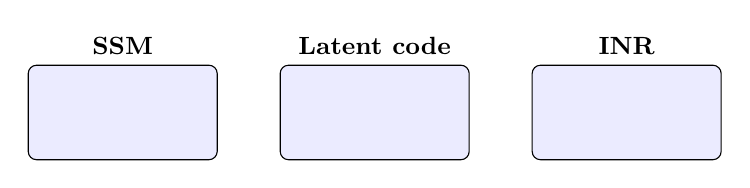
\begin{tikzpicture}[every node/.style={transform shape}]
  % symmetric tiles (continuous fill) behind each icon -- content is centred on each origin
  \foreach \x in {0,3.2,6.4}{
    \draw[rounded corners=3pt, fill=blue!8] (\x-1.2,-0.6) rectangle (\x+1.2,0.6);
  }
  \node[font=\bfseries\small] at (0,0.85)   {SSM};
  \begin{scope}[shift={(0,0)}]   \iconSSM    \end{scope}
  \node[font=\bfseries\small] at (3.2,0.85) {Latent code};
  \begin{scope}[shift={(3.2,0)}] \iconLatent \end{scope}
  \node[font=\bfseries\small] at (6.4,0.85) {INR};
  \begin{scope}[shift={(6.4,0)}] \iconINR    \end{scope}
\end{tikzpicture}
\end{document}
